\section{Introducción}
\section{Amenazas y desafios}
\section{Soluciones e iniciativas}

Desde la publicación del manifiesto de la Budapest OA Initiative \cite{boai} en 2002, han surgido distintas iniciativas que tratan de promover la publicación científica en acceso abierto. Estos estímulos proceden de distintas fuentes, tanto del ámbito gubernamental como el editorial, e incluso de personas concretas cuyos proyectos han afectado al curso del acceso libre a la ciencia.

\subsection{Iniciativas investigadoras}

Diferentes editoriales han puesto en marcha la creación de revistas de acceso abierto (\textit{Open Access Journals, OAJ}). El primer OAJ fue \textit{New Horizons in Adult Education} de la editorial Wiley \cite{earlyoaj}, fundado en 1987. Le siguieron \textit{Psycoloquy} y \textit{Public Access-Computer Systems Review} en 1989. A partir de 1990, fueron surgiendo más OAJs de forma incremental. En la actualidad, el \textit{Directory of Open Access Journals}, creado y mantenido originalmente por la universidad de Lund \cite{nordic}, \footnote{Disponible en \url{https://doaj.org/}, accedido el 29 de noviembre de 2017.} contabiliza un total de 10544 revistas de acceso abierto. En la fig.~\ref{fig:doaj} se muestra el total de OAJs que se han puesto a disposición pública en el directorio a lo largo del tiempo. Se puede observar que el crecimiento se acentúa progresivamente conforme avanzan los años.

\begin{figure}[htbp]
  \centering
  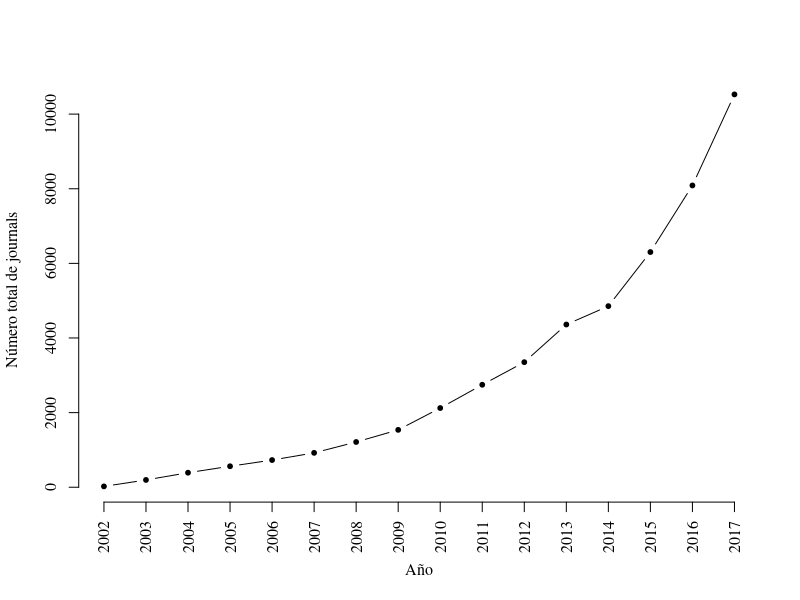
\includegraphics[width=0.8\textwidth]{doaj_years.png}
  \caption{\label{fig:doaj}Total de OAJs listados en el \textit{Directory of Open Access Journals} desde su creación en 2002. Datos de \url{https://doaj.org/csv}}
  
\end{figure}

Otra de las iniciativas que han marcado un impacto en el progreso del acceso abierto ha sido el boicot a editoriales y lobbies anti-Open Access, como Elsevier \cite{costknowledge}. En particular, una de las acciones más dañinas fue la renuncia del equipo editorial al completo del conocido journal \textit{Lingua} de Elsevier sobre lingüística, para después fundar un nuevo OAJ orientado a la misma temática, \textit{Glossia} \cite{linguaglossia}.

%- BioMed Central
%- Nucleic Acids Research (OUP)
%- Molecular Systems Biology (Nature)

\subsection{Legislación a favor de Open Access}

Holanda, Noruega, UE \cite{enserink2016dramatic}

\subsection{Iniciativas independientes}

Swartz, Sci-Hub

\section{Conclusiones}

Antes de la era de la información y tecnología, el rol de las revistas científicas era múltiple. El principal era la divulgación de las investigaciones científicas. Las revistas cobraban el coste de la maquetación, el cual no era sencillo para matemáticas, el coste de publicar en formato físico y el de distribución de los mismos a los suscriptores. En la era digital, nada de esto supone un coste tan elevado.

https://www.theguardian.com/science/2017/jun/27/profitable-business-scientific-publishing-bad-for-science
